\section{Evaluation}\label{evaluation}
This section will contain an evaluation of \pyt{}.
First the vulnerabilities described in \cref{security_vulnerabilities} will be run and serve as proof that the tool catches these vulnerabilities.
Thereafter \pyt{} will be run on real projects and the performance of the tool will be evaluated.

\subsection{Detecting Manufactured Vulnerabilities}
In \cref{security_vulnerabilities} we presented four implementation mistakes that would leave a web application vulnerable.
In this section the resulting tool, \pyt{}, will be run on the presented examples to see if they are being detected as hoped.

\paragraph{SQL injection}
The first example was the SQL injection which can be found in \cref{appendix:sqli}.
Here we expect to find the two vulnerabilities presented in \cref{vulnerabilities:sqli}, the naive execution of the query parameter and the unescaped filter.

As seen on \cref{sqli:console} we get a report with two vulnerabilities.
The first one detected is the filtering vulnerability.
\pyt{} tells us that the trigger word 'get' was found in line 33, which then reached line 36 where the trigger word 'filter' marked it as a sink.

The second one is the naive implementation of the database query.
Here the vulnerability is reported to begin at line 26 where the trigger word 'get' pointed out a sink.
This sink then reaches line 27 where the trigger word 'execute' indicates a sink.

Both vulnerabilities were thus able to be found by \pyt{}.

\begin{figure}
  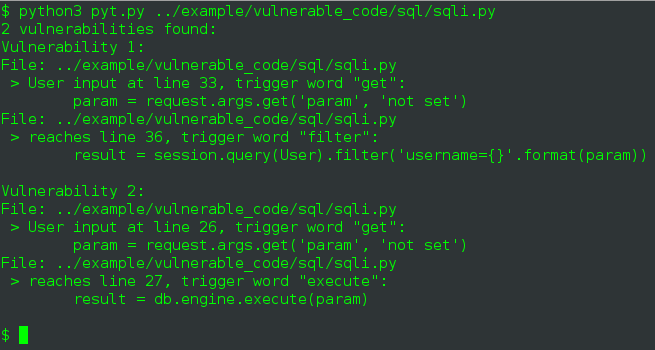
\includegraphics[width=\textwidth]{./figures/sqli_console.png}
  \caption{Running \pyt{} on the SQL injection example}
  \label{sqli:console}
\end{figure}

\paragraph{Command injection}
The next example was the command injection which can be found in \cref{appendix:command_injection}.
Here we expect to find the one vulnerability presented in \cref{vulnerabilities:ci} where the content of the form field reaches the subprocess call.

The execution of \pyt{} on the example can be seen on \cref{ci:console}.
\pyt{} reports one vulnerability being present in the application.
A source is found on line 15 with the trigger word 'form', which reaches a sink in line 18 marked because of the trigger word 'subprocess.call'.
In this case the source was assigned to a new variable in line 16 to make up the complete command to be run.
This is shown by \pyt{} as to provide information to the developer of how the tainted value did flow through the code.
  
\begin{figure}
  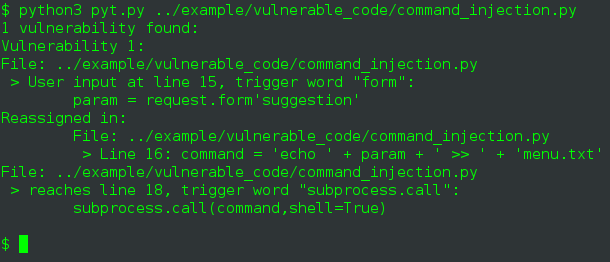
\includegraphics[width=\textwidth]{./figures/command_injection_console.png}
  \caption{Running \pyt{} on the command injection example}
  \label{ci:console}
\end{figure}

\paragraph{Cross site scripting}
The next vulnerability presented was the cross site scripting attack described in \cref{vulnerabilities:xss}.
The code can be found in \cref{appendix:xss}.

The execution of \pyt{} on the example can be seen on \cref{xss:console}.
Here a source is found in line 6 with the trigger word 'get', which reaches the sink in line 9 with the trigger word 'replace'.
Notice that the vulnerability reports a reassignment in line 10 which is irrelevant to the vulnerability because it happens after the sink.
Also notice that the reported line looks different than the source line because of the CFG representation of a return node.
This can potentially be confusing for the user of \pyt{}.

\begin{figure}
  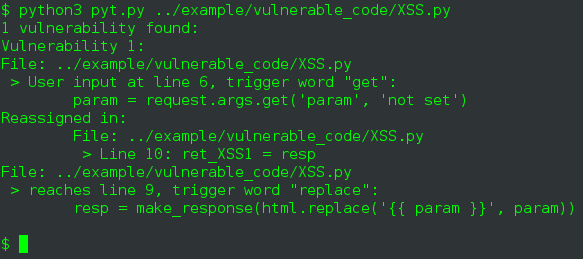
\includegraphics[width=\textwidth]{./figures/xss_console.png}
  \caption{Running \pyt{} on the XSS example}
  \label{xss:console}
\end{figure}

\subparagraph{Sanitised cross site scripting example}
As mentioned in \cref{theory_finding_vulns} some vulnerabilities can be sanitised by special functions, making the dangerous code harmless.
Running \pyt{} on the sanitised version presented in \cref{sanitised_xss} results in the output presented in \cref{xss_sanitised:console}

Here the vulnerability is found as in the above, but it concludes the vulnerability report by adding that it is potentially sanitised by the 'escape' function.

\begin{figure}
  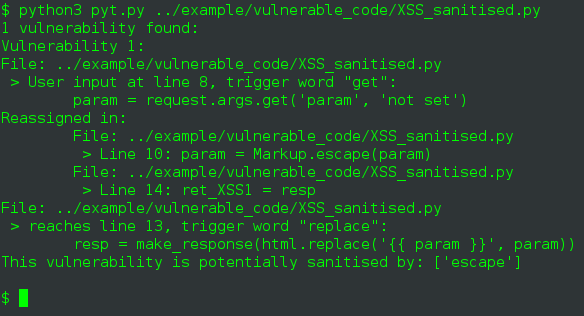
\includegraphics[width=\textwidth]{./figures/xss_sanitised_console.png}
  \caption{Running \pyt{} on the sanitised XSS example}
  \label{xss_sanitised:console}
\end{figure}

\paragraph{Path traversal}
The final vulnerability presented was the path traversal.
The code can be found in \cref{appendix:path_traversal}.
In this example we expect to find the vulnerability presented in \cref{vulnerabilities:traversal}.

The execution of \pyt{} on the example is shown in \cref{path_traversal:console}.
Here the report shows one vulnerability, starting with a sink found in line 8 with the trigger word 'get'.
This source then reaches the sink in line 11 which is detected by the trigger word 'send\_file'.

\begin{figure}
  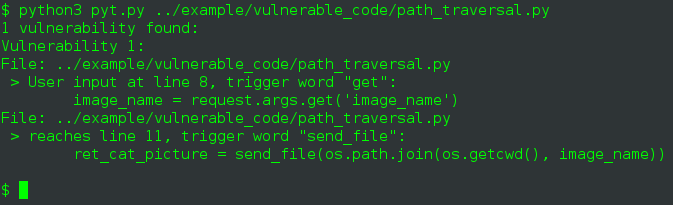
\includegraphics[width=\textwidth]{./figures/path_traversal_console.png}
  \caption{Running \pyt{} on the Path traversal example}
  \label{path_traversal:console}
\end{figure}

\subsection{Detecting Vulnerabilities in Real Projects}\label{evaluation:real}
Six open source projects were tested with \pyt{}, for evaluation its performance on realistic inputs.
A table with the results can be seen on \cref{evaluation:real:table}.

\begin{figure}
  \centering
  \begin{tabular}{|l|c|}
    \hline
    \textbf{Project} & \textbf{Vulnerabilities} \\
    \hline
    \hline
    brightonpy.org\cite{brightonpy} & 0 \\
    flask-pastebin\cite{flask_pastebin} & 0 \\
    flask\_heroku\cite{flask_heroku} & 0 \\
    guacamole\cite{guacamole} & 0 \\
    flamejam\cite{flamejam} & 0 \\
    microblog\cite{microblog} & 0 \\
    flaskbb\cite{flaskbb} & undecided \\
    \hline
  \end{tabular}
  \caption{Results.}
  \label{evaluation:real:table}
\end{figure}

As one can see on the table, no vulnerabilities were found and there were even one project where \pyt{} did not terminate.
This shows that \pyt{} can be used for real projects

\paragraph{Flaskbb}
Flaskbb did not terminate in a reasonable amount of time, and the run was manually stopped.
Upon further inspection it turns out to be due to the amount of nodes being created.
432855 nodes were created, just in the main control flow graph.
This huge amount of nodes makes the analysis takes up much time and space.

